% https://tex.stackexchange.com/a/472539
\documentclass{beamer}

\usepackage{adjustbox}
\usepackage{tikz}
\usetikzlibrary{mindmap,overlay-beamer-styles}

\begin{document}

   \begin{frame}{Title}
        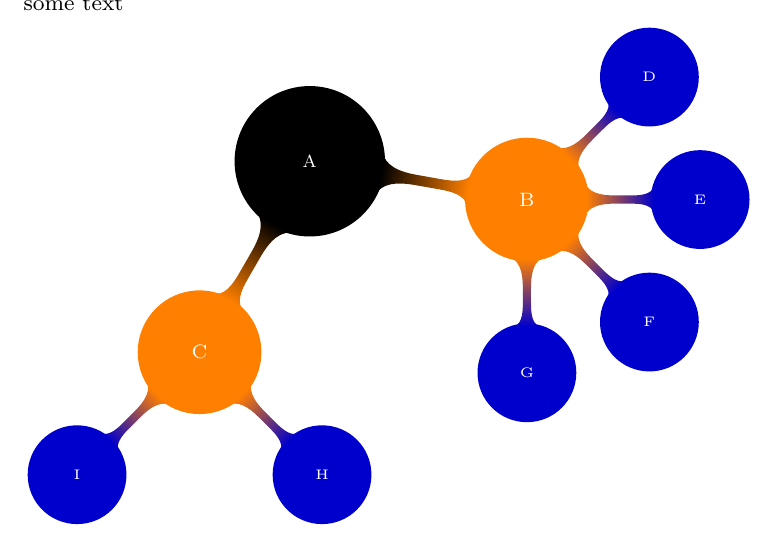
\begin{tikzpicture}[
            small mindmap,
              level 1 concept/.append style={
                sibling angle=110,
                every child/.style={concept color=orange}
              },
              level 2 concept/.append style={
                sibling angle=90,
                every child/.style={concept color=blue!80!black}
              }
              ]
          \path[concept color=black,text=white]
            node[concept,scale=0.8] {A}
            [clockwise from=-10]
            child[visible on=<2->] {
              node[concept] {B}
              [clockwise from=45]
                  child[sibling angle=45,visible on=<3->] { node[concept] {D}}
                  child[sibling angle=45,visible on=<3->] { node[concept] {E } }
                  child[sibling angle=45,visible on=<3->] { node[concept] {F}}
                  child[sibling angle=45,visible on=<3->] { node[concept] {G} }
            } 
            child[visible on=<2->] {
              node[concept] {C}
              [clockwise from=-45]
                child[visible on=<4->]{ node[concept]{ H}}
                child[visible on=<4->]{ node[concept]{ I}}
            };
            \begin{scope}[remember picture, overlay]
           \node at (-3,2) {some text};  
           \end{scope}          
        \end{tikzpicture}  
        \end{frame}

\end{document}
